\subsubsection{概要}
ツナチームは、ROS 2をベースに自作ナビゲーションスタックを作成して使用した。
%図\ref{fig:robot}の小型移動ロボット上で動作させ、
%をさせることを目的とした。
この自作ナビゲーションスタックは、
GitHub上のリポジトリuhobeike/ike\_nav\cite{ike_nav}
に公開している。
また、リポジトリの内容については
%「自作ナビゲーションスタックでつくばチャレンジ2023に挑戦してみた話」
\cite{ike_nav_detail}にまとめた。
%↑いちおう教育的観点で言うと、「記事内に金出した研究室とかその他関係者に謝辞入れやがれ自分のことしか書いてなくてよくないよこれ。」
%(言うの恥ずかしいので言わせないでほしい・・・)

このパッケージは「Nav2のような複雑な
システムではなく、シンプルで修正しやすいパッケージを作成したい」
という動機で作成した。
ソフトウェアを再利用してフィードバックすることも重要であるが、
ブラックボックスのない
ソフトウェアパッケージを開発する方針も考えられたため、
開発に踏み切った。

%例えば、つくばチャレンジ中に何か解決したい問題が発生し、
%ソフトウェア上で解決したいとなった場合に、
%パラメータやコードに対して手を入れやすいメリットがあると考えている。

%uhobeike/ike\_navの作成に関する詳細については、

%↓いらない
%\subsubsection{使用したハードウェア}
%ツナチームでは、図\ref{fig:robot}の機体を自律走行させた。
%機体には、2つのコンピュータが搭載されている。
%一つ目は、計算用として、ノートPCを搭載した。
%このノートPC上でike\_navを動作させた。
%二つ目は、機体の制御用として、Raspberry Pi 4B+を搭載した。
%
%観測用のセンサは、2次元LiDARであるUST-30LX\cite{UST-30LX}を搭載した。
%このLiDARの捜査角度は、270[deg]であり、最大検出距離は60[m]である。


\subsubsection{ike\_navのシステム構成}

図\ref{fig:tuna_system}に、ike\_navのシステム構成を示す。
ike\_navは、地図、2次元LiDARからの観測情報(スキャン)、
ロボットのオドメトリを入力して受け入れ、
ある目標地点まで到達するための速度および推定した自己位置を出力する。

\begin{figure}[h]
  \begin{center}
    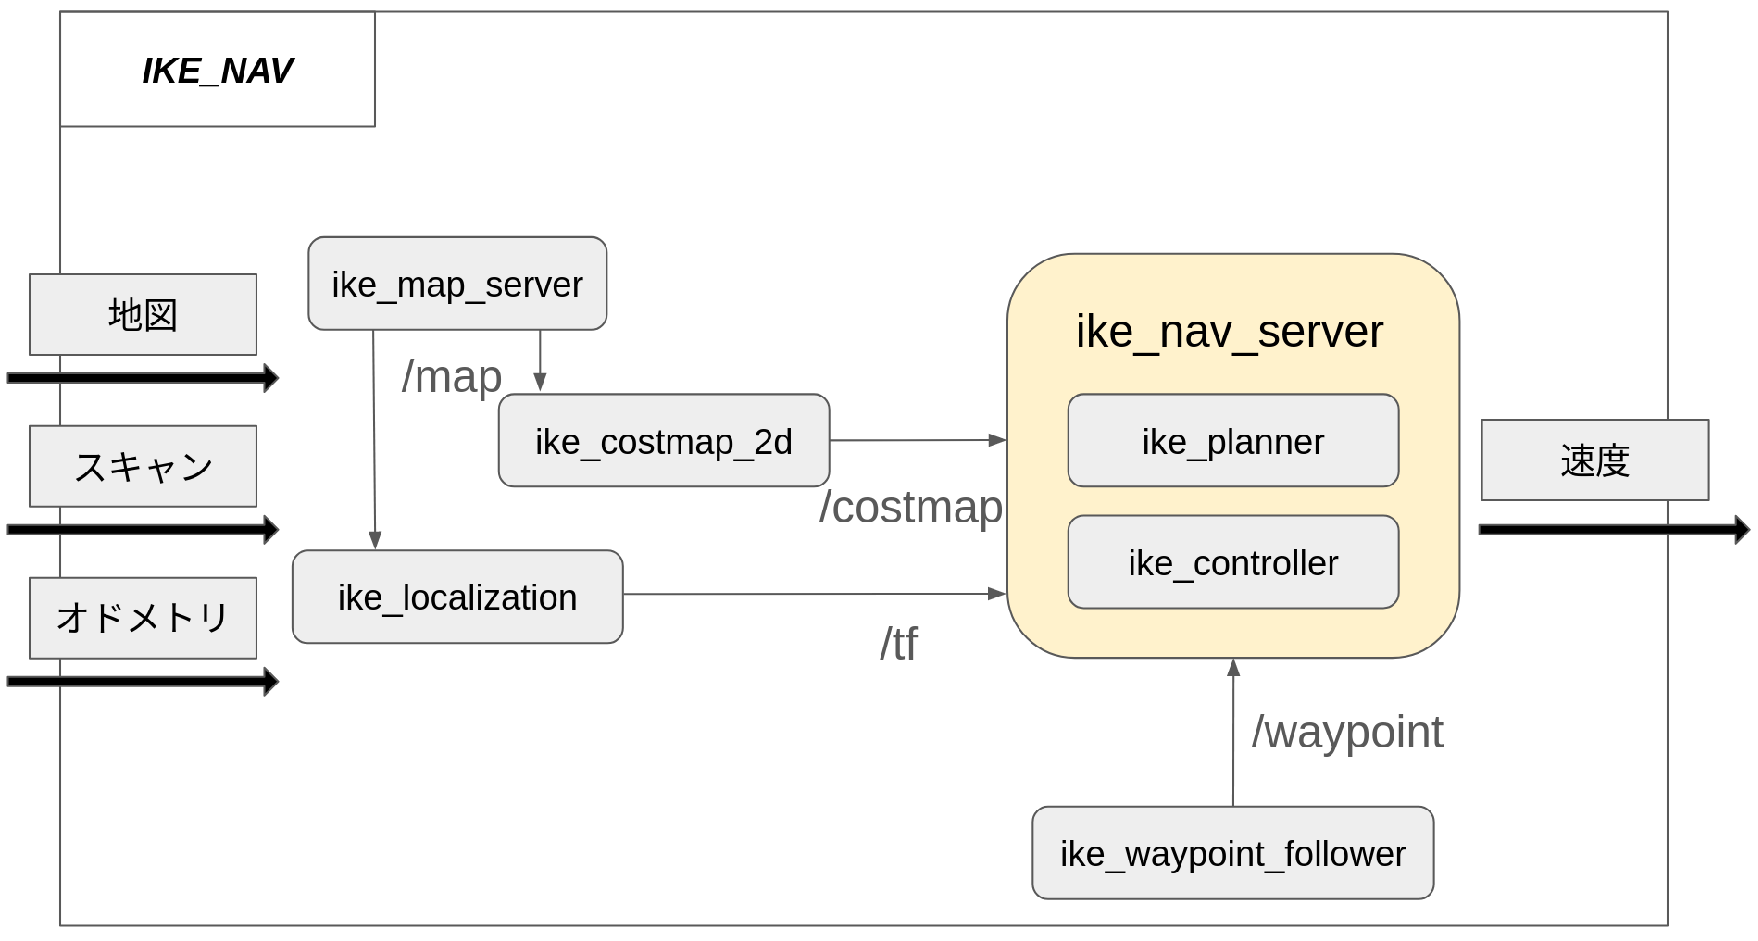
\includegraphics[width=1.0\linewidth]{figs/ike_nav.pdf}
    \caption{ツナチームのシステム構成}
    \label{fig:tuna_system}
  \end{center}
\end{figure}

ike\_navはメタパッケージであり、
自己位置推定、経路計画、経路追従などがそれぞれ別々にパッケージ化されている。
含まれるパッケージを列挙すると、次のようになる。
\begin{description}
  \item[・ike\_controller(経路追従):]経路、推定位置を入力し、速度を出力
  \item[・ike\_costmap\_2d(コストマップの管理):]地図、観測情報を入力し、コストマップを出力
  \item[・ike\_localization(自己位置推定):]観測情報、地図、ロボットのオドメトリを入力し、自己位置を出力
  \item[・ike\_map\_server(地図の管理):]pgmなどのデータからROS 2の占有格子地図を出力
  \item[・ike\_nav\_server(目標地点までの管理):]目標地点を入力し、到達するまでを管理
  \item[・ike\_planner(経路計画):]コストマップ、推定位置を入力し、経路を出力
  \item[・ike\_waypoint\_follower(複数目標地点の管理):]事前に設定した目標地点を辿るように管理
\end{description}

ike\_localization(自己位置推定)とike\_planner(経路計画)は、
それぞれつくばチャレンジでもよく用いられる
MCL(Monte Carlo Localization)\cite{fox1999etal}
とA*探索\cite{hart1968}を利用して実装した。
%最短経路を導出するアルゴリズムであり、
%他の最短経路法であるダイクストラ\cite{dijkstra1959}よりも
%速く最短経路を導出することができるため採用した。
ike\_planner(経路計画)のA*では、センサで観測した障害物
を回避する経路を導出するように実装した。
ike\_controller(経路追従)では、経路追従の手法として、
モデル予測制御(Model Predictive Control、MPC)\cite{alberto2006}を実装した。
MPCは、他の追従手法と比較して、計算コストが高いというデメリットがあるが、
経路に対する追従性が高いというメリットがあるため採用した。